\label{sec:jeffery}
The Jeffery orbits describe the motion of an ellipsoidal particle in Stokes flow. The orbits for axisymmetric ($a_x = a_z \ne a_y$) ellipsoidal particles were found by Jeffery and reformulated by Yarin \emph{et al}~\cite{Yarin} who computed orbits for asymmetric particles. The equations of motion for a triaxial particle in the form of Yarin \emph{et al} is

\begin{subequations}\label{eq:jeffrey}
\begin{align}
\frac{d\theta}{dt} 	&= (g_2 \sin \psi + g_3 \cos \psi ) \sin \theta, \\
\frac{d\phi}{dt} 	&= \tfrac{1}{2} + g_3\sin \psi - g_2 \cos \psi,\\
\frac{d\psi}{dt}	&= g_1 + (g_2\cos \psi - g_3\sin \psi) \cos \theta \\
\end{align}
\end{subequations}

where the functions  $g_i$ are defined as

\begin{subequations}
\begin{align}
g_1 &= \frac{a_y^2 - a_z^2}{2(a_y^2 + a_z^2)} 
		\left(-\tfrac{1}{2}(\cos^2 \theta + 1 )\sin 2\phi \sin 2\psi + \cos\theta \cos 2\phi \cos 2\psi \right), \\
g_2 &= \frac{a_z^2 - a_x^2}{2(a_x^2 + a_z^2)}
		\left( -\cos\theta \sin 2\phi \sin\psi  +  \cos 2\phi \cos\psi \right), \\
g_3 &= \frac{a_x^2 - a_y^2}{2(a_x^2 + a_y^2)}
		\left( \cos\theta \sin 2\phi \cos\psi + \cos 2\phi \sin\psi \right).
\end{align}
\end{subequations}

where $(\phi, \theta, \psi)$ are the Euler angles seen in figure \ref{fig:eulerangles} and . 

Looking at figure \ref{fig:orbitparams} we see that $n_x$ and $n_y$ have periodic orbits, we call each one of these periodic changes a flip. The period of flipping $T$ is for an axisymmetric particle \cite{Jeffery}

\begin{equation}\label{eq:flipRate}
T = 2\pi \left( \lambda + \frac{1}{\lambda} \right)\frac{1}{\kappa},
\end{equation}

\noindent where $\kappa$ is the shear rate. 

Solutions to the equations of motions can be found with numerical methods as shown by Yarin \cite{Yarin}. Note that the eq. \ref{eq:jeffrey} uses the coordinates from Yarin which differ from the ones used in this thesis in the same way as is discusse in Johansson \cite{AntonThesis}. The time evolution of $\theta$ and $\psi$ for different initial conditions can be plotted in a Poincaré map, also known 
as a Surface-of-Section (S.O.S.) \cite{poincare}. This plots the $\psi$ and $\theta$ coordinates each time $\phi = 0$. The points for every initial condition is bound to a certain region of such a map called the orbit. A few such maps are shown in Figure \ref{fig:orbitmaps}

For a particle with an $\epsilon \in \left[0.01-0.05\right]$ there are essentially three classes of orbits based on the initial condition $\theta_0$.

\begin{enumerate}
\item \textbf{Periodic}: $\left|\theta_0\right| \approx 1$ in which there is little variation and the particle is largely periodic with fluctuations too small to measure.
\item \textbf{Quasi-periodic sign preserving}: For $\left|\theta_0\right|> \theta_b$ the amplitude of $\cos(\theta)$ changes noticeably but does not change sign. $\theta_b$ is some breaking point that changes for different $\epsilon$
\item \textbf{Quasi-periodic sign changing}: For small $\left|\theta_0\right|$ the amplitude of $\cos(\theta)$ will change noticeably and change in sign from positive to negative.
\end{enumerate}

For larger asymmetries $\epsilon > 0.05$ there are chaotic orbits that appear as areas with dots. Chaotic orbits can been seen around the quasi-periodic circular orbits in figure \ref{fig:orbitmap4} where they appear as a 'sea' of dots.

Simulations of these three different types of orbits are illustrated in figure \ref{fig:orbittypes} both on the S.O.S. as well as the in components of $\mathbf{n}$ as a function of time. We can see that while $n_x$ and $n_y$ are periodic, albeit with different amplitudes, the 
behaviour of $n_z$ is significantly different. For the $n_z \approx 1$  orbit shown in green it is constant on the S.O.S and is simply periodic over time. For the sign presercing quasi-periodic orbit in red it is bent on the S.O.S and we can see in the time series that it is doubly periodic as it peaks with a fixed period but the amplitude of the peaks vary periodically themselves. For the sign changing quasi-periodic orbit in blue $n_z$ changes sign, again with a fixed period.


%\begin{figure}[H]
%\centering
%\begin{subfigure}[b]{0.45\textwidth}
%\includegraphics[width=0.9\textwidth]{figures/method/channelDetail.pdf}
%\caption{Sketch of the channel}\label{fig:channelsketch}
%\end{subfigure}
%\begin{subfigure}[b]{0.45\textwidth}
%\includegraphics[width=0.9\textwidth]{figures/method/ChannelZoomed.jpg}
%\caption{Picture of the channel}\label{fig:channelpicture}
%\end{subfigure}
%\caption{A sketch of the channel as well as a picture of the channel as it is set up during a measurement. The channel is only 150 $\mu$m deep, but the PDMS surrounding it is around 15 mm to try and prevent the channel from expanding and contracting too much.}
%\label{fig:channel}
%\end{figure}


\begin{figure}[H]
\centering
\begin{subfigure}[b]{0.45\textwidth}
\includegraphics[width=\textwidth]{figures/theory/map.pdf}
\caption{A poincare map}\label{fig:orbitmap}
\end{subfigure}\hspace{1em}%
\begin{subfigure}[b]{0.5\textwidth}
\includegraphics[width=\textwidth]{figures/theory/orbit.pdf}
\caption{The time series for the components \\ of the unit vector.}\label{fig:orbitparams}
\end{subfigure}
\caption{A Poincare map and three different orbits for a simulated particle with $\lambda=7$ and $\epsilon=0.05$. The three orbits highlight the three different kinds of motion, the quasi-periodic sign changing orbit in blue, the quasi-periodic sign preserving orbit in red and the periodic orbit in green. We see that while $n_x$ and $n_y$ look qualitatively similar but differ in amplitude for the different orbits, $n_z$ shows three different types of behaviour}
\label{fig:orbittypes}
\end{figure}



\begin{figure}[H]
\centering
\begin{subfigure}[3a]{0.40\textwidth}
\includegraphics[width=\textwidth]{figures/theory/7-1-1.pdf}
\caption{Poincare map for $\lambda = 7, \epsilon = 0$.}\label{fig:orbitmap1}
\end{subfigure}\hspace{1em}%
\begin{subfigure}[3b]{0.40\textwidth}
\includegraphics[width=\textwidth]{figures/theory/7-1o01-1.pdf}
\caption{Poincare map for $\lambda = 7, \epsilon = 0.01$.}\label{fig:orbitmap2}
\end{subfigure} \\
\begin{subfigure}[3a]{0.40\textwidth}
\includegraphics[width=\textwidth]{figures/theory/7-1o05-1.pdf}
\caption{Poincare map for $\lambda = 7, \epsilon = 0.05$.}\label{fig:orbitmap3}
\end{subfigure}\hspace{1em}%
	\begin{subfigure}[3b]{0.40\textwidth}
\includegraphics[width=\textwidth]{figures/theory/7-1o25-1.pdf}
\caption{Poincare map for $\lambda = 7, \epsilon = 0.25$.}\label{fig:orbitmap4}
\end{subfigure} 
\caption{Four Poincare maps for different $\epsilon$. Already at $\epsilon = 0.01$ there are noticeably quasi-periodic 
orbits around the centre at $\cos(\theta) \approx \psi \approx 0$ but it is also a significantly larger region for $\epsilon = 0.05$. For $\epsilon = 0.25$ we can see chaotic orbits surrounding the circular orbits in the centre that appear as a 'sea' of dots. Note that some wavelike pattern can appear to exist in the figure \ref{fig:orbitmap2} and  \ref{fig:orbitmap2}, this is caused by aliasing/compression issues with printing several curved lines close together.}\label{fig:orbitmaps}
\end{figure}

\subsection{Winding number} \label{sec:winding}
The quasi-periodic orbits are also referred to as double-periodic~\cite{Yarin}. This to emphasize the fact that the amplitude of the short period $\theta_2$ also varies periodically with period $\theta_1$. The ratio between the two periods is referred to as the winding number $\omega$

\begin{equation}\label{eq:winding}
\omega = \frac{\theta_1}{\theta_2}.
\end{equation}

\noindent The winding number of the quasi-periodic sign preserving orbit from figure \ref{fig:orbittypes} is illustrated in Figure \ref{fig:windingDef}.

\begin{figure}[H]
\begin{center}
\includegraphics[width=0.7\textwidth]{figures/theory/WindingNrFixed2.pdf}
\end{center}
\caption{The $n_z$ sign preserving quasi-periodic orbit from figure \ref{fig:orbitparams} over a longer time, highlighting the short period $\theta_2$ which is simply the period of $\phi$ and the longer period $\theta_1$. The winding number is defined as the ratio between the longer and shorter periods.}
\label{fig:windingDef}
\end{figure}

%This can also be thought of as the number of intersections on the surface of section before coming back to the initial condition, divided by the number of laps. A lap for a circular orbit is a rotation around the center whereas for a flat orbit it is moving along length of the orbit. asdasd, see figure MAKE A FIGURE. 
This number is the same for any point along a given orbit on a poincare map but changes for different orbits as well as for different asymmetries. The winding numbers for orbits along $\psi=0$ for $\epsilon=\{0.01, 0.05, 0.10\}$ can be seen in figure \ref{fig:windingdifferent}. This shows us that if we can measure the winding number it allows us to approximate the asymmetry of the particle.  This is done by looking at the difference in winding number between a quasi-periodic sign preserving orbit and a sign changing orbit. This is useful in order to differentiate between particles of different asymmetry, because they can have similar orbits but very distinct winding number. 
 
\begin{figure}[H]
\begin{center}
\includegraphics[width=0.7\textwidth]{figures/theory/WindingTrend.png}
\end{center}
\caption{The winding number as a function of $\cos(\theta)$ for three different asymmetries. The sharp edge that occurs centered around zero is where the sign changing orbits end and sign preserving orbits begin. We see that a lower asymmetry leads to a sharper difference between the sign changing and the sign preserving orbits.}
\label{fig:windingdifferent}
\end{figure}
